\subsection{Implementierung von Pyro(J)}
\label{sec:pyroJ}
PyroJ ist der Optimierer, der von \cite{shanbhag2014optimizing} für die Prüfung der Vollständigkeit von Pellenkofts Regelmenge RS-B2 genutzt wurde. Dies wird im folgenden Kapitel genauer beschrieben. Ebenfalls wurde auf Basis dieses Optimierers die neue Regelmenge RS-Graph implementiert und getestet. 
PyroJ basiert auf dem von \cite{roy2001multi} in C++ implementierten Optimierer Pyro und wurde automatisch von C++ nach Java übersetzt. Der Optimierer Pyro wurde nach dem Vorbild des Volcano Optimierers entwickelt. Volcano wurde als Vorbild gewählt, da es sich bei Volcano um einen hoch-respektierten, state-of-the-art, regelbasierten Optimierer handelt, der auch die Basis von kommerziellen Datenbanksytemen wie MS SQL Server ist. Gerade die Erweiterbarkeit im Hinblick auf das Datenmodell, Executionsmodell und die Möglichkeit Transformationsregeln und Operatoren hinzuzufügen, sollten übernommen werden.


Einige Unterschiede zwischen Volcano und Pyro bestehen jedoch aus Sicht von \cite{roy2001multi}:

\subsubsection{Trennung zwischen logischem und physischem Planspace}

Pyro generiert zuerst logische Pläne, die dann in physische Pläne umgesetzt werden. In einem dritten Schritt kann daraus der optimale Plan ausgewählt werden. Diese Schritte werden nacheinander unabhängig ausgeführt. In der Realität können diese drei Schritte überlappen. So ist es möglich, dass zuerst für einen logischen Plan alle physischen Pläne erzeugt werden und dann aus diesen Plänen nur der günstigste behalten wird. Daraufhin kann dann der nächste logische Plan erzeugt und für ihn der günstigste physische Plan gesucht werden. Nur wenn dieser günstigste Plan billiger ist als der bisher gefundene Plan, wird der physische Plan auch weiterhin gespeichert. Dieser Ansatz kann Ressourcen-schonender sein, als der in Pyro verwendete Ansatz, bei dem immer alle Daten vorgehalten werden. 

\subsubsection{Vereinigung von Äuqivalenten-Subausdrücken}

Bei Volcano ist es möglich gewesen, dass mehrere Äquivalenzklassen den selben Knoten repräsentieren. Beispielsweise kommt in der Anfrage $(A \Join B \Join C) \cup (B \Join C \Join D)$ $B$ und $C$ zweimal vor. Obwohl dies der Fall ist, werden für $B$ und für $C$ je zwei Äquivalenzklassen erzeugt. Nachdem diese beiden Relationen als unabhängig betrachtet werden, fällt auch nicht auf, dass der Ausdruck $B \Join C$ mehrfach vorkommt und somit auch in einer Äquivalenzklasse behandelt werden kann. Später wurde dieses Problem bei Volcano erkannt und mit Hilfe einer Memofunktion gelöst.

Auch Pyro(J) implementiert eine solche Memofunktion, die die Wiederverwendung von bekannten Äuqivalenzklassen erlaubt.


\subsubsection{Generierung mit Description-Files}

Ein fundamentaler Unterschied zwischen Volcano und Pyro auf den von \cite{roy2001multi} nicht hingewiesen wird, ist die Erstellung des Optimierers. Bei Pyro handelt es sich um einen fertigen Optimierer, der nicht mehr generiert werden muss. Es sind keine Description-Files vorhanden. Eine einfache Konfiguration ist nicht mehr möglich. Eine Generierung eines Optimierers findet überhaupt nicht statt.


\subsubsection{Ausführung der Experimente}


\begin{figure}[ht]
  \centering
  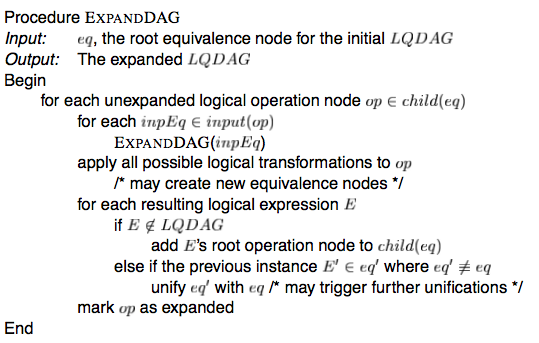
\includegraphics[scale=0.75]{02_Related_Work/ExpandDAG.png}
  \caption{Pseudocode: ExpandDAG}
  \label{ExpandDAG}
\end{figure}

Auf PyroJ wurden von \cite{shanbhag2014optimizing} Experimente zur Überprüfung der Pellenkoft Regelmengen durchgeführt. Die Durchführung der Tests geschah mit Hilfe des Expanders \texttt{ExpandDAG}. Die Prozedur (vgl. Abb. \ref{ExpandDAG}) expandiert basierend auf einem Äquivalenzknoten unterschiedliche Transformationen aus und speichert diese in Äquivalenzklassen. Der Algorithmus, der von \cite{roy2001multi} implementiert wurde sieht vor, dass in jeder Äquivalenzklasse über die Menge der bisher noch nicht expandierten Planknoten iteriert wird. Falls die dem Planknoten untergeordneten Äquivalenzklassen bisher noch unbekannt sind, werden diese Äquivalenzklassen expandiert. Sobald alle untergeordneten Pläne expandiert wurden, werden die Regeln auf den aktuellen Planknoten angewendet. Neue alternativen werden der bestehenden Äquivalenzklasse untergeordnet.

\cite{roy2001multi} legt außerdem in einem Beweis dar, dass dieser Algorithmus für RS-B1 mit Prädikatpushdown (vgl. Kapietl 3) vollständig ist und alle Pläne gefunden werden können. 

Wie im folgenden Kapitel beschrieben, wurden unterschiedliche Regelmengen auf ihre Vollständigkeit und Performance getestet. Außerdem wurde eine neue Regel implementiert. 
